%
% directionfield.tex -- Template für standalone TIKZ Bilder
%
% (c) 2019 Prof Dr Andreas Müller, Hochschule Rapperswil
%
\documentclass[tikz,12pt]{standalone}
\usepackage{amsmath}
\usepackage{times}
\usepackage{txfonts}
\usepackage{pgfplots}
\usepackage{csvsimple}
\usetikzlibrary{arrows,intersections,math}
\begin{document}
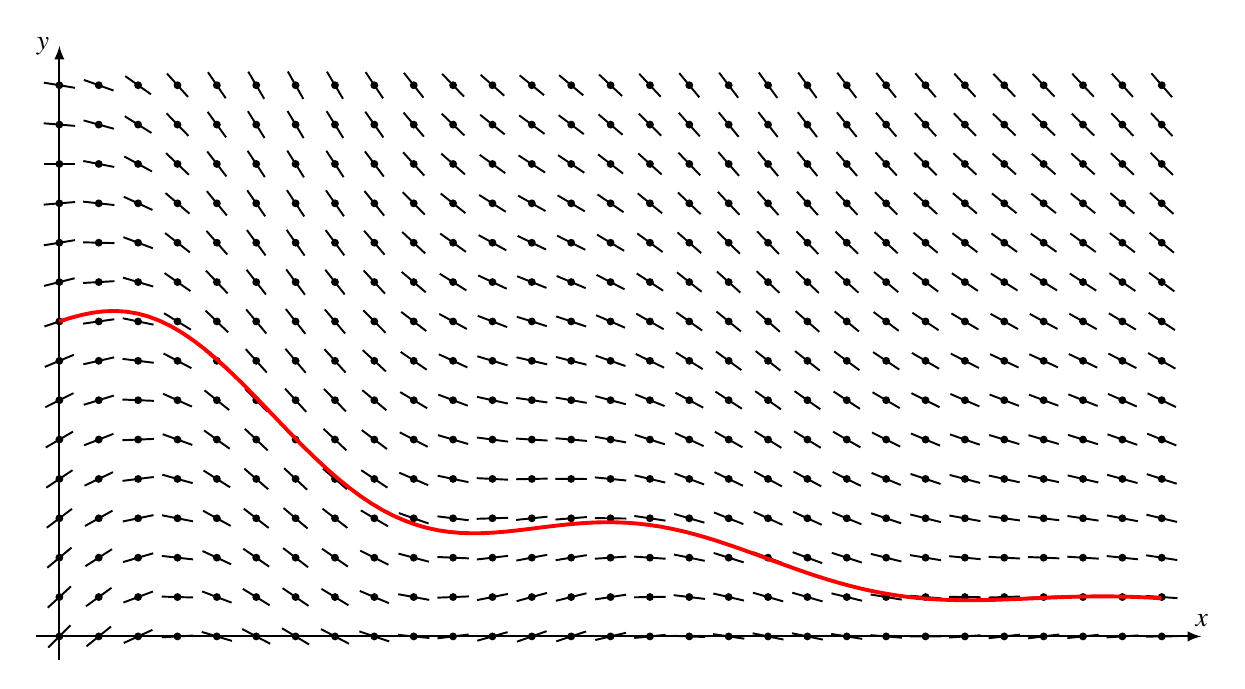
\begin{tikzpicture}[>=latex]

\def\r{0.2}

\def\richtung#1#2#3{
	\fill ({#1},{#2}) circle[radius=0.05];
	\draw[line width=0.7pt]
		({#1+\r*(1/sqrt(1+#3*#3))},{#2+\r*(#3/sqrt(1+#3*#3))})--
		({#1-\r*(1/sqrt(1+#3*#3))},{#2-\r*(#3/sqrt(1+#3*#3))});
}

\draw[->,line width=0.7pt] (-0.3,0)--(14.5,0) coordinate[label={$x$}];
\draw[->,line width=0.7pt] (0,-0.3)--(0,7.5) coordinate[label={left:$y$}];

\foreach \x in {0,0.5,...,14}{
	\foreach \y in {0,0.5,...,7}{
		\richtung{\x}{\y}{(-(\y/6)+exp(-\x/6)*cos(\x*(180/3.14159)))}
		%\richtung{\x}{\y}{(-\y/6)}
	}
}
\def\c{4}

\draw[color=red,line width=1.4pt] plot[domain=0:14,samples=100]
	({\x},{exp(-\x/6)*(\c+sin(\x*(180/3.14159)))});

\end{tikzpicture}
\end{document}

